\documentclass{article}

\usepackage{fullpage}
\usepackage{parskip}
\usepackage{setspace}
\usepackage{mathtools}
\usepackage{tikz}
\usetikzlibrary{arrows}
\usetikzlibrary{decorations.markings}
\usetikzlibrary{calc}
\usepackage{standalone}
\usepackage{float}
\usepackage{caption}
\usepackage{subcaption}
\usepackage{amsmath}
\usepackage{amsfonts}
\usepackage{amsthm}
\usepackage[ruled]{algorithm2e}
\usepackage{adjustbox}
\usepackage{enumerate}
\usepackage[nocompress]{cite}
\usepackage{hyperref}
\usepackage{booktabs}

\newtheorem{theorem}{Theorem}
\newtheorem{proposition}{Proposition}


\title{Extensions to Markov Models of One Node Deadlocking Queueing Networks - Baulking \& Scheduled Vacations}
\author{Cindy Huang, Vincent Knight, Geraint Ian Palmer}
\date{}


\begin{document}
\onehalfspacing

\maketitle

\section{Introduction}

This chapter contains collaborative work done jointly by Cindy Huang, Dr. Vincent Knight and myself, during Cindy's Nuffield research placement \cite{nuffieldresearchplacements} at the School of Mathematics, Cardiff University. At the time, Cindy was a sixth form student undertaking a four week placement with myself and Dr. Knight. The work involved extending the Markov chain models previously in built in Chapter~\ref{chp:markovmodelsofdeadlock}, in order to model baulking behaviour by the customers, and scheduled vacations of the servers.


\section{Baulking}

Baulking behaviour is when customers arrive, but choose not to join the queue as
the queue is too long. This decision to baulk however is probabilistic. This
% Can you add more about the basis of this, so something like:
% As is the case in a lot of the literature cite{x, y, z, ...}, the baulking
% decision is probabilistic.
work looks investigates a model of baulking discussed in
\cite{anckergafarian63}, in which arriving customers baulk with probability
$b(x)$ dependent on $x$ the number of customers already at the node. This
probability density function is shown in Equation~\ref{eqn:probbaulking}.

\begin{equation}\label{eqn:probbaulking}
    b(x) = \left\{ \begin{array}{rr}
    0 & \text{if } x = 0\\
    1 - \frac{\beta}{x} & \text{otherwise}
    \end{array} \right.
\end{equation}

where $n$ is the number of customers already at the node, and $0 < \beta \leq 1$ is some measure of willingness to join the queue. Figure~\ref{fig:examplebaulkingfunctions} shows how the baulking function $b(x)$ behaves for different values of $x$ and $\beta$.
% Can we change x to m
The more customers there are at the node already, the more likely a newly arriving customer is to baulk. The higher the value for $\beta$ the less likely a newly arriving customer is to baulk, or the more willing they are to join the queue despite there being customer ahead of them.

\begin{figure}
    \begin{center}
        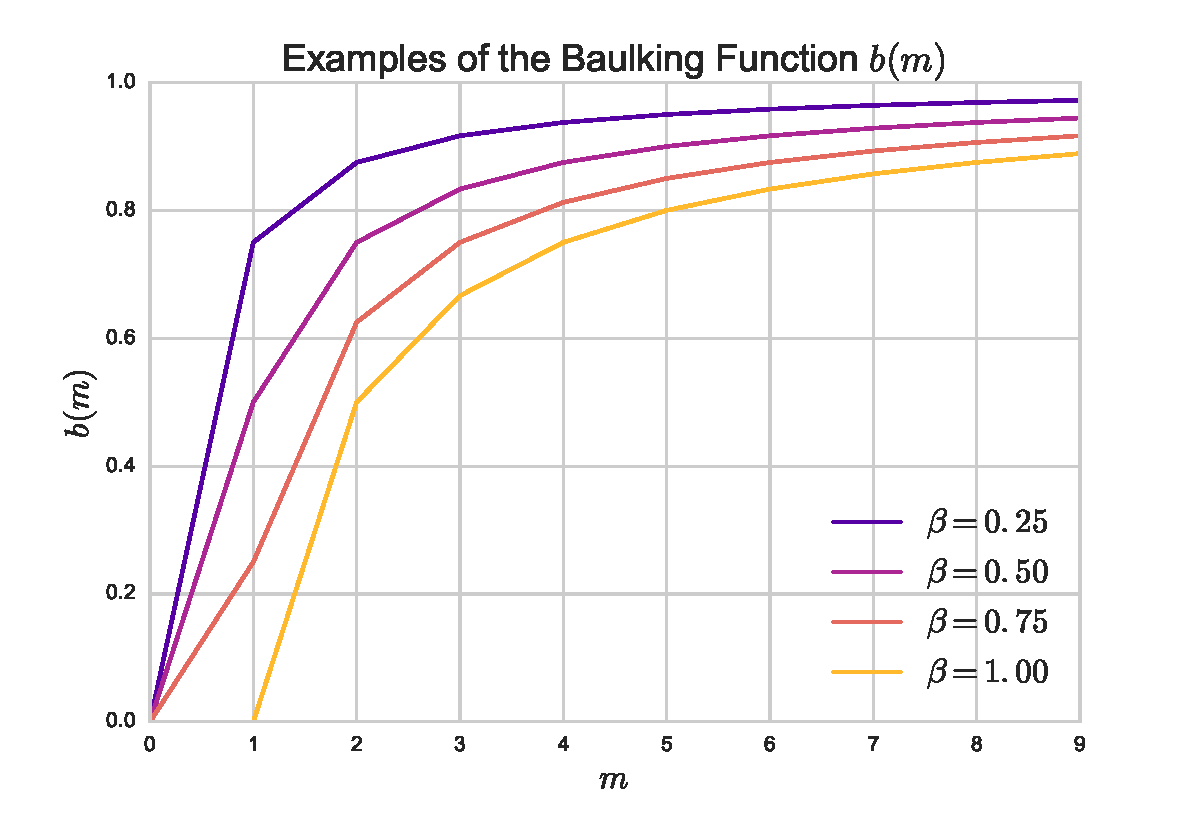
\includegraphics[width=0.7\textwidth]{img/examplebaulking.pdf}
    \end{center}
    \caption{Behaviour of the baulking function $b(n)$ for different values of $\beta$.}
    \label{fig:examplebaulkingfunctions}
\end{figure}


\subsection{Markov Chain Model of One Node Queueing Network with Baulking}

Consider the one node queueing network shown in Figure~\ref{fig:onenodenetwork_baulking}.
Customers arrive to the system at a rate $\Lambda$, but baulk with probability $1 - b(x)$ when there are $x$ customers already at the node, and so join the queue with probability $b(x)$. There is one server, who serves customers at a rate of $\mu$, and there is only capacity for $n$ customers to wait in the queue. After service there is a probability $r_{11}$ of rejoining the queue, and so a probability $1-r_{11}$ of exiting the system after service.

\begin{figure}
    \begin{center}
        \includestandalone[width=\textwidth]{img/1nodeexample_baulking}
    \end{center}
    \caption{A one node queueing network with baulking.}
    \label{fig:onenodenetwork_baulking}
\end{figure}

% This state space comes a bit out of nowhere: The state space for the
% corresponding Markov chain is given by:
The state space is given by:
        \[S = \{i\in\mathbb{N} \nonscript\; | \nonscript\; 0 \leq i \leq n + 1
        \}\cup\{(-1)\}\]
where \(i\) denotes the number of individuals in service or waiting, and $(-1)$ denotes the deadlocked state.

Define $\delta = i_2 - i_1$ for all $i_k \geq 0,\; k\in{1, 2}$.
The transitions are given by Equations~\ref{eqn:1nssAb}, \ref{eqn:1nssBb} and \ref{eqn:1nssCb}.

\begin{equation}\label{eqn:1nssAb}
  q_{i_1, i_2} = \left\{
  \begin{array}{rr}
    \left. \begin{array}{rr}
      \Lambda & \text{if } i_1 = 0 \\
      \frac{\Lambda \beta}{i_1} & \text{if } 0 < i_1 < n + 1 \\
      0 & \text{otherwise}
    \end{array} \right\} & \text{if } \delta = 1 \\
    (1 - r_{11})\mu & \text{if } \delta = -1 \\
    0 & \text{otherwise}
  \end{array} \right.
\end{equation}

\begin{equation}\label{eqn:1nssBb}
  q_{i, (-1)} = \left\{
  \begin{array}{rr}
    r_{11}\mu & \text{if } i = n + 1 \\
    0 & \text{otherwise}
  \end{array}
  \right.
\end{equation}

\begin{equation}\label{eqn:1nssCb}
  q_{-1, i} = 0
\end{equation}

The Markov chain is shown in Figure~\ref{fig:1nodeMCbaulking}.

\begin{figure}[!htbp]
  \begin{center}
    \includestandalone[width=0.75\textwidth]{img/markov_chain_1node_baulking}
  \end{center}
  \caption{Diagrammatic representation of the Markov chain for the one node system with baulking.}
  \label{fig:1nodeMCbaulking}
\end{figure}

The only difference between this Markov model and the model presented in Chapter~\ref{chp:markovmodelsofdeadlock} is that the rate at which customers enter the queue now varies with the number of customers already in the system. If there are $x$ customers in the system ($x > 0$) then the rate at which customers join the queue is $\frac{\Lambda \beta}{x}$.
Note that for any $0 < \beta \leq 1$, and for any number of customers $x$, there is always a positive probability of a customer joining the queue, and therefore it is always possible to reach the deadlock state. If however $\beta = 0$ was chosen, then the only possibility of a customer joining the queue is when $x = 0$, and so the system will never reach deadlock.

Figure~\ref{fig:varybeta} shows the effect of varying the baulking parameter $\beta$ on times to deadlock. Base parameters of $\Lambda = 3$, $n = 2$, $\mu = 3$, and $r_{11} = 0.6$ are used.
The behaviour observed here is intuitive, as $\beta$ increases, the time to deadlock decreases. Interpreting $\beta$ as the willingness of newly arriving customers to join the queue, then as this parameter increases more newly arriving customers join the queue, and so the queueing capacity fills up quicker. The baulking parameter $\beta$ therefore has a very similar effect on the time to deadlock as the arrival rate $\Lambda$.
% I think the above paragraph could be broken up in to smaller sentences.
% The rate at which the occupancy increases, increases.

\begin{figure}
    \begin{center}
        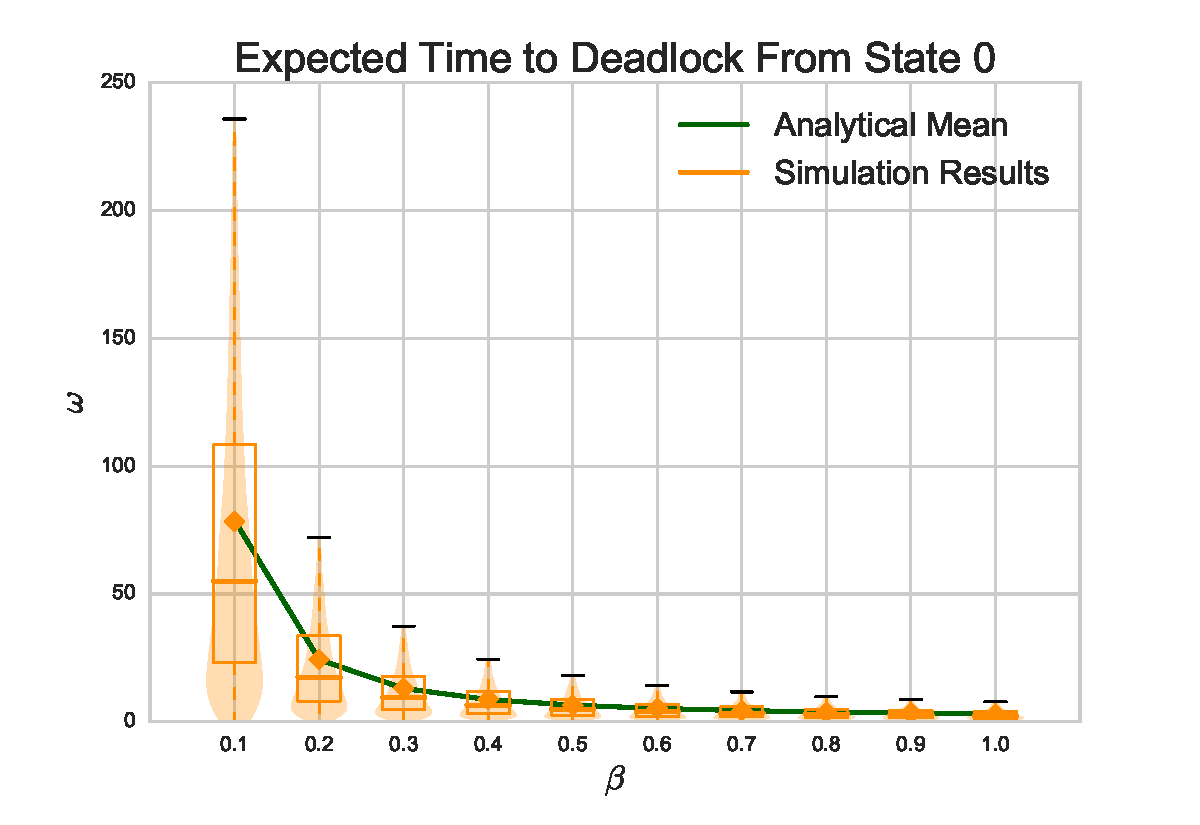
\includegraphics[width=0.6\textwidth]{img/vary_beta.pdf}
    \end{center}
    \caption{Time to deadlock of the one node baulking network, analytical \& simulation results (10,000 iterations), varying $\beta$.}
    \label{fig:varybeta}
\end{figure}

Let's investigate the combined effect of $\beta$ along with other parameters on the time to deadlock.
Figures~\ref{fig:varyLambdabybeta} and \ref{fig:varybetabyLambda} show the effects that the baulking parameter $\beta$ has on the time to deadlock as the arrival rate $\Lambda$ varies, and also how this effect is affected by the arrival rate.
Figures~\ref{fig:varyr11bybeta} and \ref{fig:varybetabyr11} show the effects that the baulking parameter $\beta$ has on the time to deadlock as the transition probability $r_{11}$ varies, and also how this effect is affected by the transition probability.
All three parameters, $\Lambda$, $r_{11}$, and $\beta$ have similar effects on the time to deadlock; as these parameters are increased, then the queueing capacity if filled up more quickly, and so we get to a situation where blocking, and deadlock, can occur sooner. Therefore increasing these parameters decreases the time to deadlock.
Combining these parameters results in an amplified effect.

\begin{figure}
\begin{center}
\begin{subfigure}[b]{0.45\textwidth}
    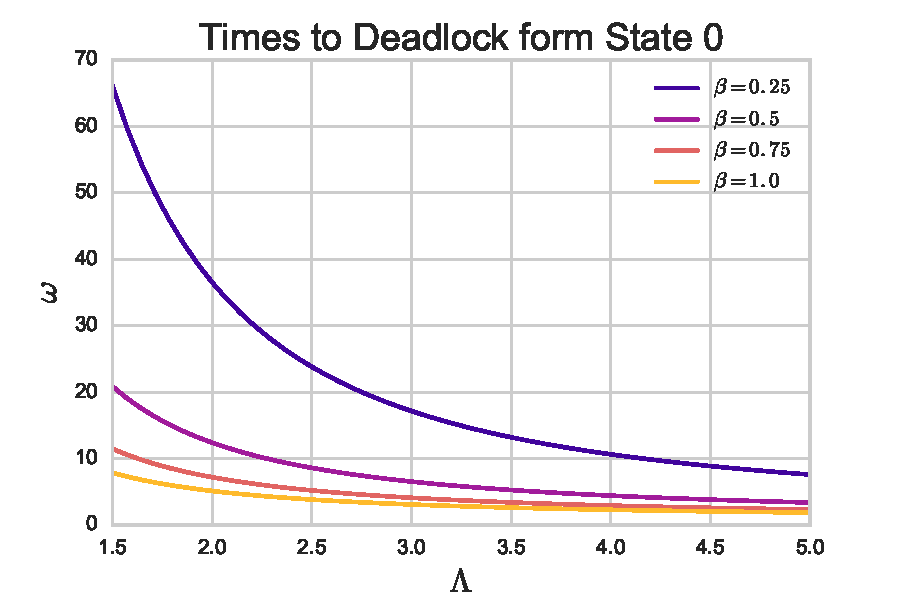
\includegraphics[width=\textwidth]{img/varylambda_bybeta.pdf}
    \caption{Time to deadlock varying $\Lambda$ by $\beta$.}
    \label{fig:varyLambdabybeta}
\end{subfigure}
\begin{subfigure}[b]{0.45\textwidth}
    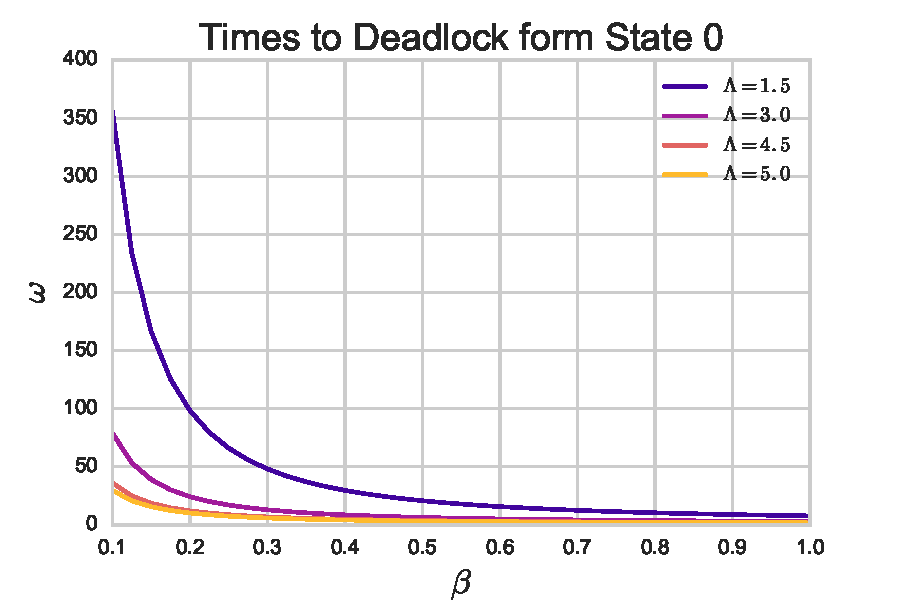
\includegraphics[width=\textwidth]{img/varybeta_bylambda.pdf}
    \caption{Time to deadlock varying $\beta$ by $\Lambda$.}
    \label{fig:varybetabyLambda}
\end{subfigure}
\end{center}
\caption{Investigating how the combined effect of the baulking parameter $\beta$ and the arrival rate $\Lambda$ on the time to deadlock.}
\label{fig:combinedeffect_betalambda}
\end{figure}

\begin{figure}
\begin{center}
\begin{subfigure}[b]{0.45\textwidth}
    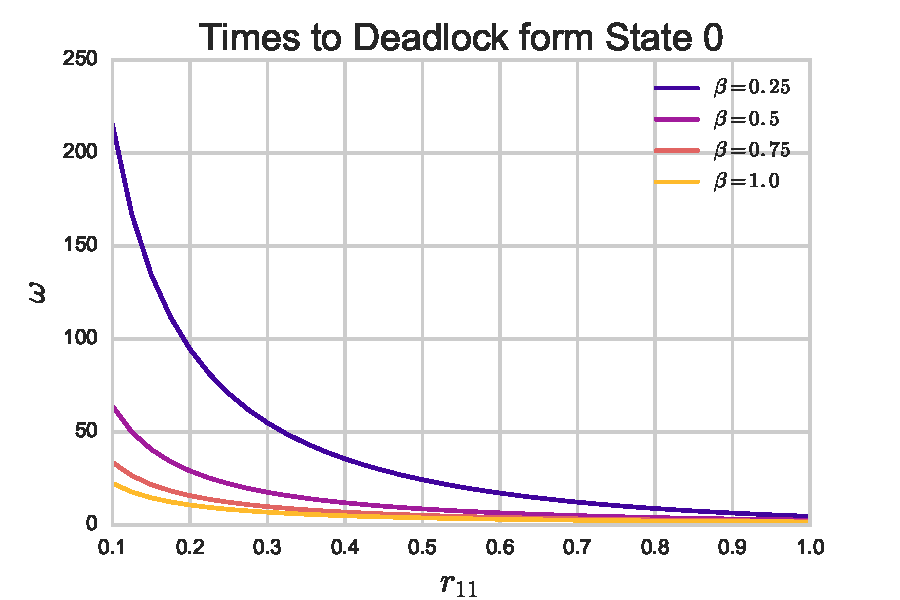
\includegraphics[width=\textwidth]{img/varyr11_bybeta.pdf}
    \caption{Time to deadlock varying $r_{11}$ by $\beta$.}
    \label{fig:varyr11bybeta}
\end{subfigure}
\begin{subfigure}[b]{0.45\textwidth}
    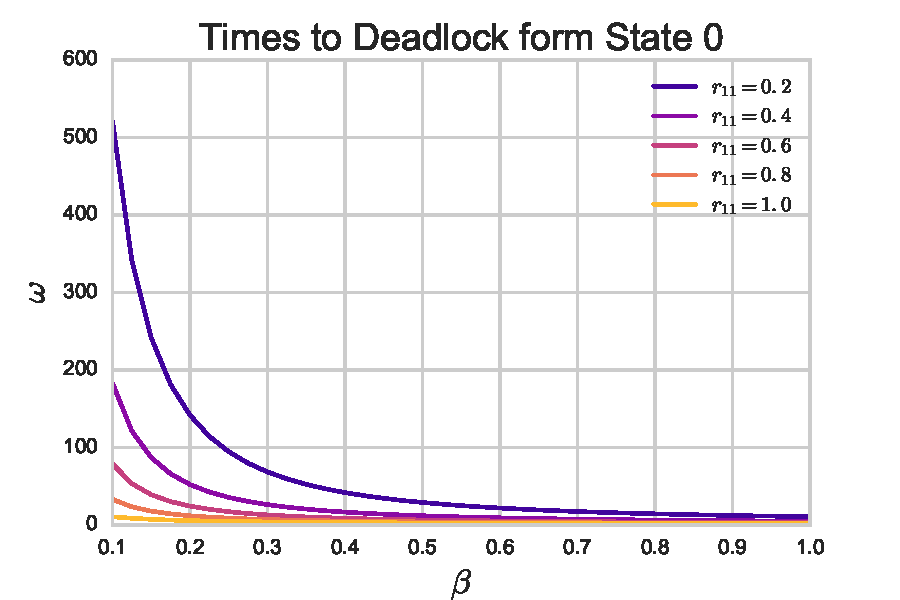
\includegraphics[width=\textwidth]{img/varybeta_byr11.pdf}
    \caption{Time to deadlock varying $\beta$ by $r_{11}$.}
    \label{fig:varybetabyr11}
\end{subfigure}
\end{center}
\caption{Investigating how the combined effect of the baulking parameter $\beta$ and the transition probability $r_{11}$ on the time to deadlock.}
\label{fig:combinedeffect_betar11}
\end{figure}

Figures~\ref{fig:varynbybeta} and \ref{fig:varybetabyn} show the effects that the baulking parameter $\beta$ has on the time to deadlock as the queueing capacity $n$ varies, and also how this effect is affected by the queueing capacity.
In Chapter~\ref{chp:markovmodelsofdeadlock} it was shown that, without baulking, as the queueing capacity increased the time to deadlock also increased, as it took longer to fill up a larger queueing capacity. This effect is also seen with baulking, however the baulking exaggerates this effect; the lower the baulking parameter $\beta$ (that is, the more likely customers are to baulk) the more exaggerated this effect. This is because the baulking function $b(x)$ is independent of $n$, and even when customers are most willing to join the queue ($\beta = 1.0$) once there are $4$ customers in the system three-quarters of arriving customers baulk. Therefore increasing $n$ makes it less and less likely for a customer to join the queue, and so more and more difficult to fill up the queue, especially when the number of customers already at the queue approaches the queueing capacity.
% Don't talk about filling up capacity. Talk about increasing occupancy.


\begin{figure}
\begin{center}
\begin{subfigure}[b]{0.45\textwidth}
    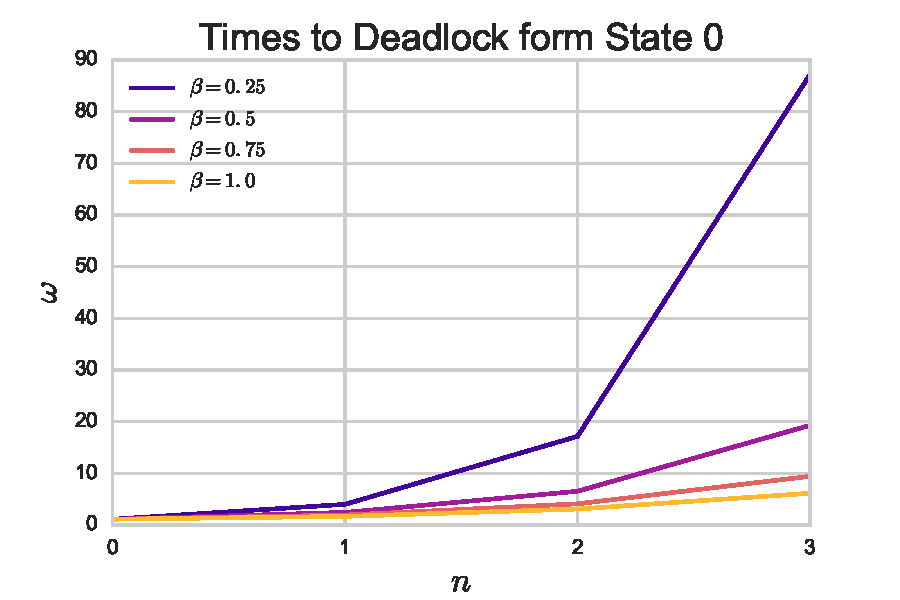
\includegraphics[width=\textwidth]{img/varyn_bybeta.pdf}
    \caption{Time to deadlock varying $n$ by $\beta$.}
    \label{fig:varynbybeta}
\end{subfigure}
\begin{subfigure}[b]{0.45\textwidth}
    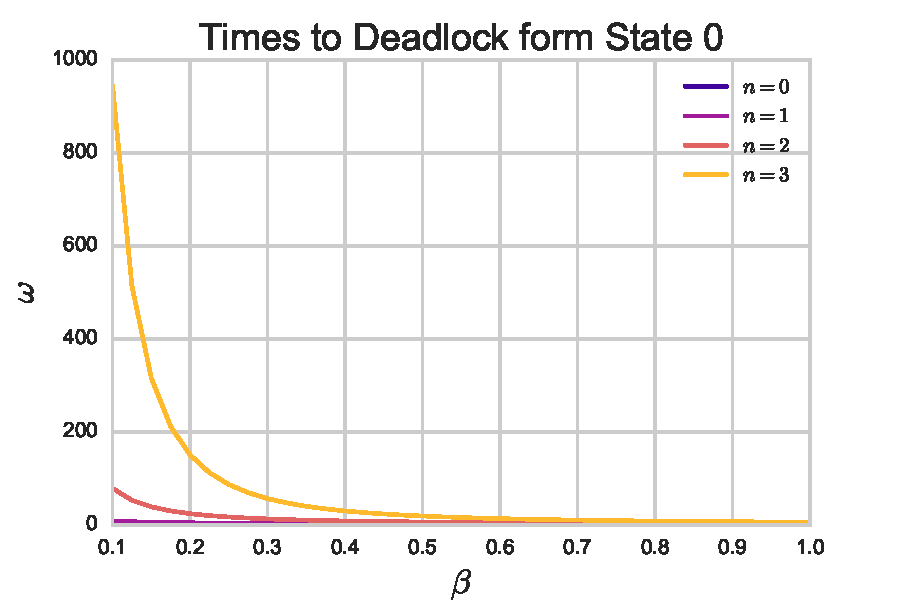
\includegraphics[width=\textwidth]{img/varybeta_byn.pdf}
    \caption{Time to deadlock varying $\beta$ by $n$.}
    \label{fig:varybetabyn}
\end{subfigure}
\end{center}
\caption{Investigating how the combined effect of the baulking parameter $\beta$ and the queueing capacity $n$ on the time to deadlock.}
\label{fig:combinedeffect_betan}
\end{figure}

Figures~\ref{fig:varymubybeta} and \ref{fig:varybetabymu} show the effects that the baulking parameter $\beta$ has on the time to deadlock as the service rate $\mu$ varies, and also how this effect is affected by the service rate.
When looking at the equivalent system without baulking in Chapter~\ref{chp:markovmodelsofdeadlock} a bowl shaped curve was observed in the time to deadlock when varying the service rate, and the presence of some service rate threshold that changes the behaviour of $\omega$. This behaviour is still present when customers exhibit baulking, however the baulking parameter $\beta$ effects the shape of the curve. Note that only the gradient of the slope for values $\mu > \hat{\mu}$, that is service rates greater that the threshold that is effected. This is because at service rates lower than $\hat{\mu}$ we assume that the system is saturated, that is that the queueing capacity is full or is filled up fast enough that the time which it is not full or negligible. Therefore in these situations the arrival rate, and so the baulking rate, cannot affect the time to deadlock, only the service rate and transition probabilities can.

Looking at the inverse plot, the effect that the service rate $\mu$ has on the time to deadlock as $\beta$ varies, Figure~\ref{fig:varybetabymu}, an interesting effect occurs. At low values of $\beta$ the greater the service rate the longer it takes to reach deadlock, however this effect is flipped at high values of $\beta$. At low $\beta$ not many customers join the queue (compared to a low $\beta$), and so a long service time in necessary to allow the queueing capacity to fill up, therefore a lower $\mu$ will yield quicker times to deadlock. At high values of $\beta$ many customers join the queue (compared to a a $\beta$), and so there is no need to wait for the queue to fill up, we can assume this will happen anyway. Therefore a lower service rate $\mu$ will cause longer for a blockage to occur that a higher service rate, and so a longer time to deadlock.

\begin{figure}
\begin{center}
\begin{subfigure}[b]{0.45\textwidth}
    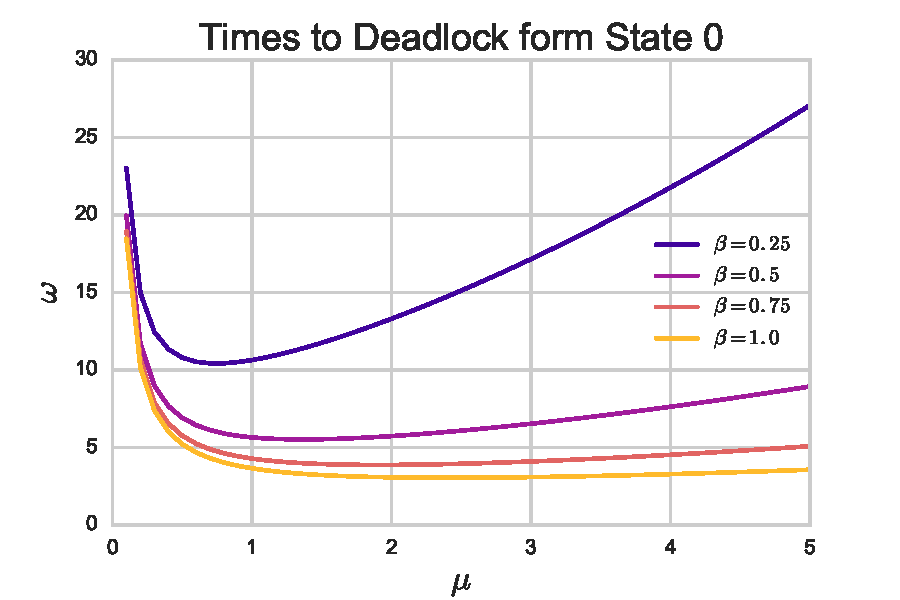
\includegraphics[width=\textwidth]{img/varymu_bybeta.pdf}
    \caption{Time to deadlock varying $\mu$ by $\beta$.}
    \label{fig:varymubybeta}
\end{subfigure}
\begin{subfigure}[b]{0.45\textwidth}
    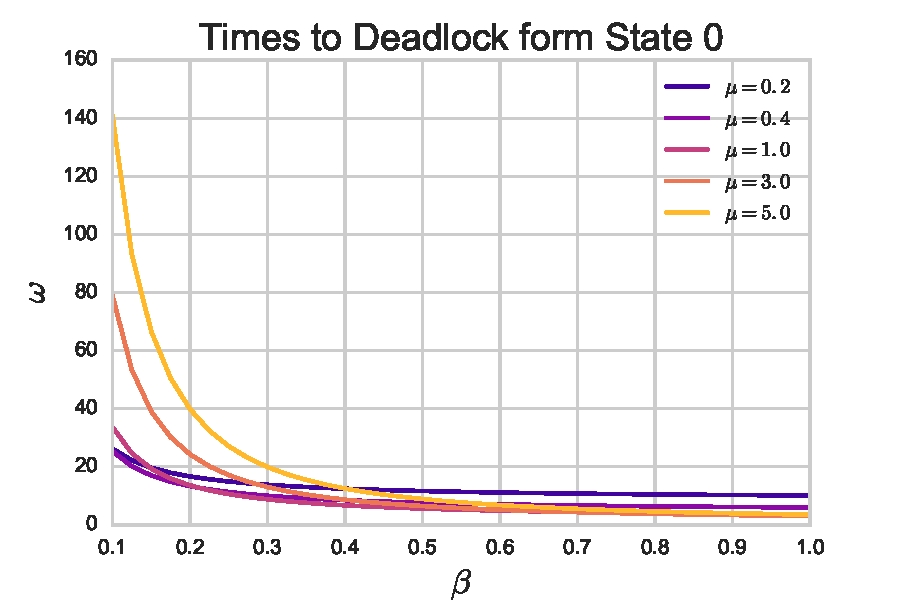
\includegraphics[width=\textwidth]{img/varybeta_bymu.pdf}
    \caption{Time to deadlock varying $\beta$ by $\mu$.}
    \label{fig:varybetabymu}
\end{subfigure}
\end{center}
\caption{Investigating how the combined effect of the baulking parameter $\beta$ and the service rate $\mu$ on the time to deadlock.}
\label{fig:combinedeffect_betamu}
\end{figure}

Figure~\ref{fig:betathreshold} shows the effect of the baulking parameter $\beta$ on the service rate threshold.
As the baulking parameter is closely associated with the arrival rate $\Lambda$,
similarly to the effect of $\Lambda$ on $\hat{\mu}$, the threshold increases as
the baulking parameter increases. This is due to a high baulking parameter means that more customers join the queue, and so it takes a larger service rate to escape the saturated zone. This relationship is not linear, and becomes less linear as the queueing capacity $n$ decreases.
% Less linear is not very rigorous. Convexity increases perhaps.

\begin{figure}[!htbp]
  \begin{center}
    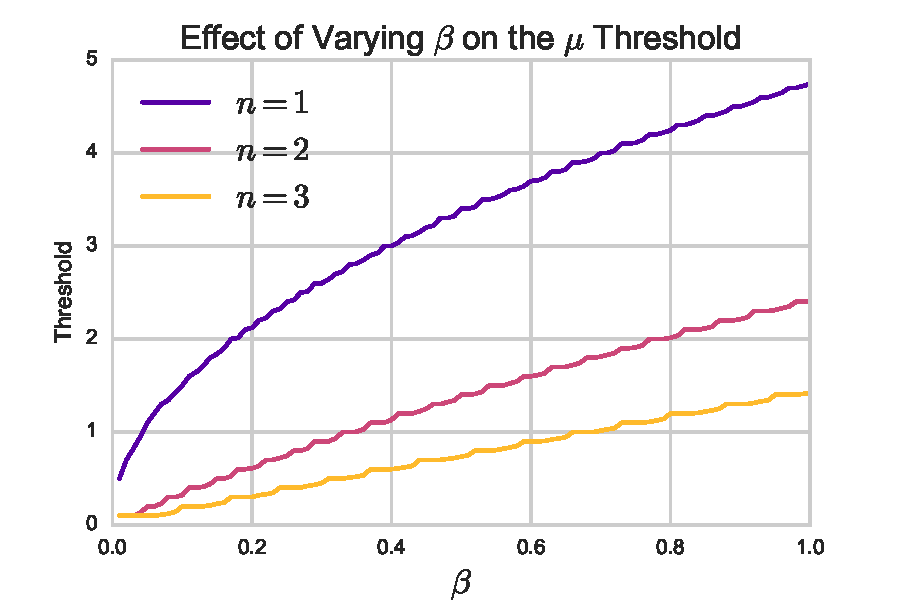
\includegraphics[width=0.75\textwidth]{img/thresholdbeta_plot}
  \end{center}
  \caption{The effect of $\beta$ on the service rate threshold $\hat{\mu}$.}
  \label{fig:betathreshold}
\end{figure}



\section{Scheduled Vacations}

% Add some literature here.
This section will extend the Markov chain model of a one node restricted queueing network discussed in Chapter~\ref{chp:markovmodelsofdeadlock}, so that server behaviour may be incorporated.
The behaviour we will focus on is scheduled vacations.
That is, the server will periodically cycle on and off duty. While the server is on duty the system behaves as usual, however when the server is off duty no services can occur, although arrivals happen as usual. When a server goes off duty, the current service is interrupted, and resumed when the server comes back on duty.

Let us call $s$ the time on duty, and $s_v$ the time on vacation. Therefore the cycle length is $s + s_v$.
% A picture would be nice here

As an example, imagine an on-line shop where orders can arrive to a queue at any
time of the day or night. The shop hires one server who processes orders from
9am to 5pm, seven days a week. From 5pm to 9am next day, that server is off duty
and no orders can be processed, however orders continue to arrive. That server
is on a scheduled vacation. (Note: if the server is mid way through processing
an order at 5pm, then they will complete that service before going off duty). Here $s$ is the time on duty (9am - 5pm), and $s_v$ the time on vacation (5pm - 9am). The cycle length is one day.

This will be modelled using time inhomogeneous Markov chains. Before we begin, a result on discretising time inhomogeneous Markov chains is required.

\subsection{Discretising Time Inhomogeneous Markov Chains}

A well known result \cite{stewart09} on discretising continuous Markov chains is that the matrix $P = Q \Delta t + I$ is a stochastic matrix if the following condition is satisfied:

\begin{equation}
\Delta t \leq \frac{1}{\max_i |q_{ii}|}
\end{equation}

This discrete Markov chain $P$ is equivalent to the continuous Markov chain $Q$ with transitions only occurring a at the discrete time interval $\Delta t$.

It is also known that if a time inhomogeneous Markov chain can be described by a transition matrix $P_1$ for the first time step, and transition matrix $P_2$ at the second time step, where $P_1$ and $P_2$ have the same states and same time steps, then that system's state can be described by the transition matrix $P_1 P_2$ for the first two times steps. This is equivalent to a time homogeneous Markov chain described by $P$, can be described by $P^n$ for the first $n$ time steps.
% A matrix does not have steps. I don't understand that part (same states and
% time steps)

How about a continuous time inhomogeneous Markov chain that is described by $Q_1$ for the first $s_1$ time units, and by $Q_2$ for the next $s_2$ time units? How can we discretise these in order to obtain transient solutions to this discretised time inhomogeneous Markov chain? Theorem~\ref{thrm:discretisetimeinhomogeneousmarkovchains} discusses this discretisation.
\newline

\begin{theorem}\label{thrm:discretisetimeinhomogeneousmarkovchains}
Given a time inhomogeneous Markov chain that is described sequentially by the continuous transition matrices $Q_j$ for $s_j$ time units, $s_j \in \mathbb{Z}$, for $j \in J = \left\{ 1, 2, ..., m \right\}$, then the discretised system requires the discretised transition matrices $P_j = Q_j \Delta t + I$, where

$$
\Delta t = \frac{\gcd_j(s_j)}{\left\lceil \frac{\gcd_j(s_j)}{\min_j \bar{\delta}_j} \right\rceil}
$$

where $\bar{\delta}_j = \frac{1}{\max_i |q_{ii}|}$, with $q_{ii}$ being the diagonal entries in the transition matrix $Q_j$.
\end{theorem}

\begin{proof}
The discretised system requires a single time step, $\Delta t$.
$\Delta t$ must be chosen such that each continuous transition matrix is discretised using $P_j = Q_j \Delta t + I$, and such that $\Delta t$ can be multiplied an integer amount of times to give all $s_j$, for $j \in J$.

First we require that $Q_j \Delta t + I$ is a stochastic matrix for each $j \in J$. In order for this to be true, we must have

\begin{equation*}
\Delta t \leq \frac{1}{\max_j |q_{ii}|} \forall\; j \in J
% Pet hate of mine: always need space after the forall. Find all of these.
\end{equation*}

where $q_{ii}$ are the diagonal entries of $Q_j$. Defining $\bar{\delta}_j = \frac{1}{\max_j |q_{ii}|} \forall j \in J$, we have that

\begin{equation}\label{eqn:cond1}
\Delta t \leq \min_j \bar{\delta}_j
\end{equation}.

Now $\Delta t \in \mathbb{R}$, but as we require that $\Delta t$ can be
multiplied by integers to give each of $s_j$ for $j \in J$, then we force
$\Delta t \in \mathbb{Q}$. Therefore $\exists\; k, m \in \mathbb{Z}$ such that $k \Delta t = m$.
% Same comment as forall
Now we have an integer $m$ that must divide each $s_j$ for $j \in J$. For
computational efficiency, we take the largest such $m$, and so $m = \gcd_j (s_j)$. Therefore, we have $\Delta t$ of form

\begin{equation}\label{eqn:cond2}
\Delta t = \frac{\gcd_j(s_j)}{k}
\end{equation}.

combining the conditions (~\ref{eqn:cond1}) and (~\ref{eqn:cond2}), we get $k$ such that
% I notice you use Equation throughout. I would change to use (x).

\begin{equation*}
\frac{\gcd_j(s_j)}{k} \leq \min_j(\bar{\delta}_j)
\end{equation*}

and so we take $k = \left\lceil \frac{\gcd_j(s_j)}{\min_j(\bar{\delta}_j)} \right\rceil$.

Finally, substituting in for $k$, we get

\begin{equation*}
\Delta t = \frac{\gcd_j(s_j)}{\left\lceil \frac{\gcd_j(s_j)}{\min_j \bar{\delta}_j} \right\rceil}
\end{equation*}

\end{proof}



\subsection{Modelling Deadlock with Servers with Scheduled Vacations}

Consider the one node restricted queueing network shown in Figure~\ref{fig:1nodescheduledvacations}.
Here customers arrive at a rate of $\Lambda$ per time unit, there is only enough room for $n$ customers to queue at a time, and after service customers rejoin the queue with probability $r_{11}$. The service rate now alternates between having $s$ time units as $\mu$, and $s_v$ time units as $0$. If a customer is in service as the service rate changes, their service is interrupted, and is resumed once the server come back on duty after $s_v$ time units on vacation.

\begin{figure}[!hbtp]
    \begin{center}
        \includestandalone[width=\textwidth]{img/1nodeexample_scheduledvacations}
    \end{center}
    \caption{A one node queueing network with scheduled vacations.}
    \label{fig:1nodescheduledvacations}
\end{figure}

This system is described by two transition matrices, $Q$ while the server is on duty, and $Q_v$ when the server is off duty.

The state space for both is given by:
        \[S = \{i\in\mathbb{N} \nonscript\; | \nonscript\; 0 \leq i \leq n + 1
        \}\cup\{(-1)\}\]
where \(i\) denotes the number of individuals in service or waiting, and $(-1)$ denotes the deadlocked state.

Define $\delta = i_2 - i_1$ for all $i_k \geq 0$. The transitions for $Q$ are given by Equations~\ref{eqn:1nssAsv}, \ref{eqn:1nssBsv} and \ref{eqn:1nssCsv}.

\begin{equation}\label{eqn:1nssAsv}
  q_{i_1, i_2} = \left\{
  \begin{array}{rr}
    \left. \begin{array}{rr}
      \Lambda & \text{if } i_1 < n + 1 \\
      0 & \text{otherwise}
    \end{array} \right\} & \text{if } \delta = 1 \\
    (1 - r_{11})\mu & \text{if } \delta = -1 \\
    0 & \text{otherwise}
  \end{array} \right.
\end{equation}

\begin{equation}\label{eqn:1nssBsv}
  q_{i, (-1)} = \left\{
  \begin{array}{rr}
    r_{11}\mu & \text{if } i = n + 1 \\
    0 & \text{otherwise}
  \end{array}
  \right.
\end{equation}

\begin{equation}\label{eqn:1nssCsv}
  q_{-1, i} = 0
\end{equation}

The transitions for $Q_v$ are given by Equations~\ref{eqn:1nssAsvv} and \ref{eqn:1nssBsvv}.

\begin{equation}\label{eqn:1nssAsvv}
  q_{i_1, i_2} = \left\{
  \begin{array}{rr}
      \Lambda & \text{if } i_1 < n \text{ and } \delta = 1 \\
      0 & \text{otherwise}
  \end{array} \right.
\end{equation}

\begin{equation}\label{eqn:1nssBsvv}
  q_{i, -1} = q_{-1, i} = 0
\end{equation}

These two cases are visualised in Figure~\ref{fig:scheduledvacationsMC}.

\begin{figure}
\begin{subfigure}[b]{\textwidth}
    \includestandalone[width=\textwidth]{img/markov_chain_1node_SV_onduty}
    \caption{Representation of $Q$, while the server is on duty.}
    \vspace{3cm}
    \label{fig:MCSVonduty}
\end{subfigure}
\begin{subfigure}[b]{\textwidth}
    \includestandalone[width=\textwidth]{img/markov_chain_1node_SV_offduty}
    \caption{Representation of $Q_v$, while the server is off duty.}
    \label{fig:MCSVoffduty}
\end{subfigure}
\caption{Diagrammatic representation of $Q$ and $Q_v$, the continuous time Markov chains describing a system with scheduled vacations while the server is on and off duty respectively.}
\label{fig:scheduledvacationsMC}
\end{figure}




Using Theorem~\ref{thrm:discretisetimeinhomogeneousmarkovchains}, these can be discretised appropriately.
As we know the structure of these Markov chains, we can simplify the theorem for this purpose.
\newline

\begin{proposition}
    % This is still a theorem.
For the one node restricted network described above, described by continuous transition matrices $Q$ for $s$ time units and $Q_v$ for $s_v$ time units, the appropriate time step to discretise the transition matrices is $\Delta t = \gcd(s, s_v) / \left\lceil \gcd(s, s_v) \left(\Lambda + (1 + r_{11}\mu\right) \right\rceil$.
\end{proposition}

\begin{proof}
From Theorem~\ref{thrm:discretisetimeinhomogeneousmarkovchains} we require
\begin{equation*}
\Delta t = \frac{\gcd_j(s_j)}{\left\lceil \frac{\gcd_j(s_j)}{\min_j \bar{\delta}_j} \right\rceil}
\end{equation*}
Now $\gcd_j(s_j) = \gcd(s, s_v)$.

For $Q$, $\bar{\delta} = 1 / \Lambda$.
For $Q_v$, $\bar{\delta} = 1 /(\Lambda + (1 - r_{11})\mu)$.
As $1 /(\Lambda + (1 - r_{11})\mu) \leq 1 / \Lambda$, for any $\Lambda \geq 0$, $0 < r_{11} \leq 1$, $\mu \geq 0$, then for any valid parameters $\min_j \bar{\delta}_j = 1 /(\Lambda + (1 - r_{11})\mu)$.

Substituting these into the original theorem yields the required result.
\end{proof}

Using this time step $Q$ and $Q_v$ can be discretised to $P$ and $P_v$ respectively.
We can now find the transient solutions, and approximate stationary solutions for this system using Equation~\ref{eqn:transientSVsolutions1}.

\begin{equation}\label{eqn:transientSVsolutions1}
\pi_{t+1} = \pi_{t} \hat{P}
\end{equation}

Where $\hat{P}$ is defined by Equation~\ref{eqn:transientSVsolutions2}.

\begin{equation}\label{eqn:transientSVsolutions2}
\hat{P} = \left\{
    \begin{array}{cc}
    P & \text{if } t \bmod (s + s_v) \leq s \\
    P_v & \text{if } t \bmod (s + s_v) > s
    \end{array}\right.
\end{equation}

In this way the probability density function, and the cumulative density function over the time steps can be found.
Figures~\ref{fig:pdfinitial} and \ref{fig:cdfinitial} show the PDF and CDF respectively of the system with parameters $\Lambda = 2.0$, $\mu = 4.0$, $n = 6$, $r_{11} = 0.2$, $s = 10$, $s_v = 5$. In the time periods where the server is on vacation, no customer can finish service, and so deadlock cannot be reached. Therefore the probability of reaching deadlock during these periods is $0$. This is observed in the PDF where the probabilities drop to $0$, and in the CDF where the cumulative probability does not increase for the duration of the vacation, at each vacation. During this vacation time, arrivals occur, but no customer leaves the queue, and so by the end of the vacation time the queue has had chance to fill up, but not empty. Therefore, immediately after a vacation period ends, the probability of deadlock shoots up as the queue will likely be in a fuller state than at the beginning of the vacation. At this point, the server returns, and so the queue begins to empty, and so the probability of deadlock decreases (although not to $0$, as the server can now send customers to rejoin the queue and cause deadlock). This results in the curved step-wise shape in the CDF, and oscillatory behaviour in the PDF that is observed.
% Are the PDF and CDF calculator analytically? Include some details.
% You can possibly include some pseudo code.
% I don't know if in previous chapters you also do stuff where you step through
% the chain until a certain number of probability is accounted for. If you do
% you should obviously mention that algorithm once and then just refer back to
% it.

\begin{figure}
\begin{center}
\begin{subfigure}[b]{0.45\textwidth}
    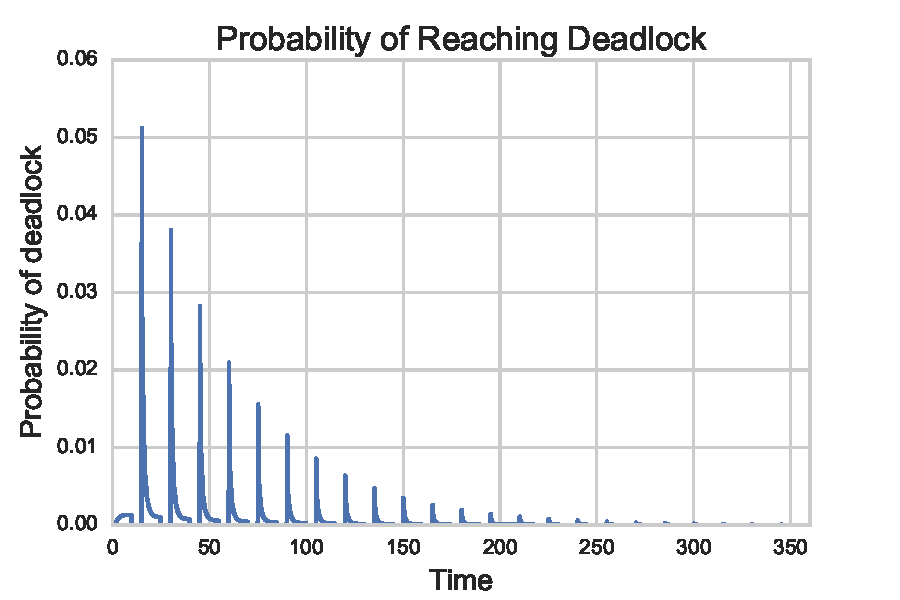
\includegraphics[width=\textwidth]{img/pdf_initial.pdf}
    \caption{Probability density function of reaching deadlock with vacations.}
    \label{fig:pdfinitial}
\end{subfigure}
\begin{subfigure}[b]{0.45\textwidth}
    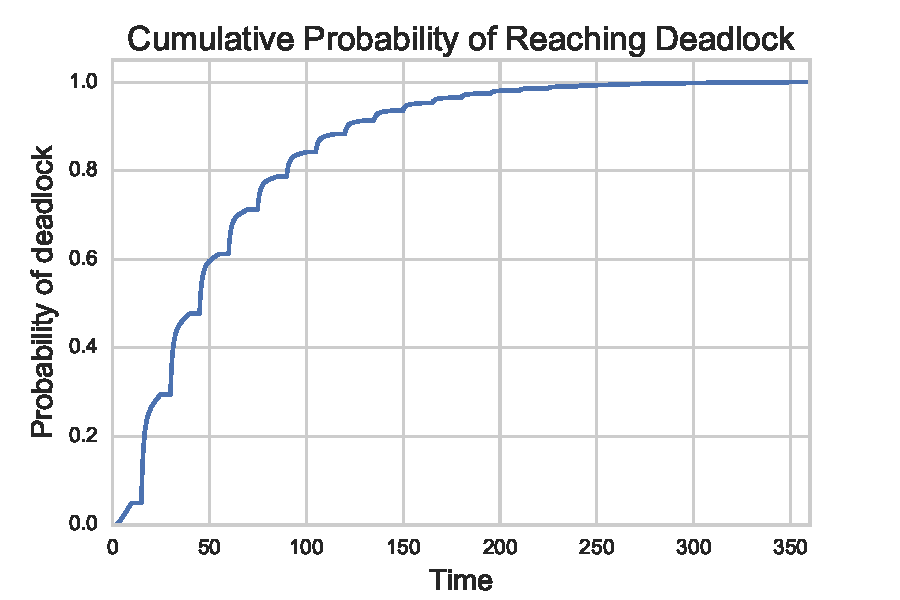
\includegraphics[width=\textwidth]{img/cdf_initial.pdf}
    \caption{Cumulative density function of reaching deadlock with vacations.}
    \label{fig:cdfinitial}
\end{subfigure}
\end{center}
\caption{PDF \& CDF of reaching deadlock in a system with scheduled vacations.}
\label{fig:pdfcdf_initial}
\end{figure}

To show that the Markov chain models agree with the simulation models, Figure~\ref{fig:scheduled_vacations_MC_simulation} shows the time to deadlock results of system with parameters $\Lambda = 5.0$, $\mu = 2.0$, $r_{11} = 0.5$, $s = 10$, and $s_v = 5$, for various values of the queueing capacity $n$. Violin and box plots show the distribution of the times to deadlock obtained using the simulation model (using Ciw), and the green line plot shows the corresponding solution from the Markov chain formulation.

\begin{figure}
\begin{center}
    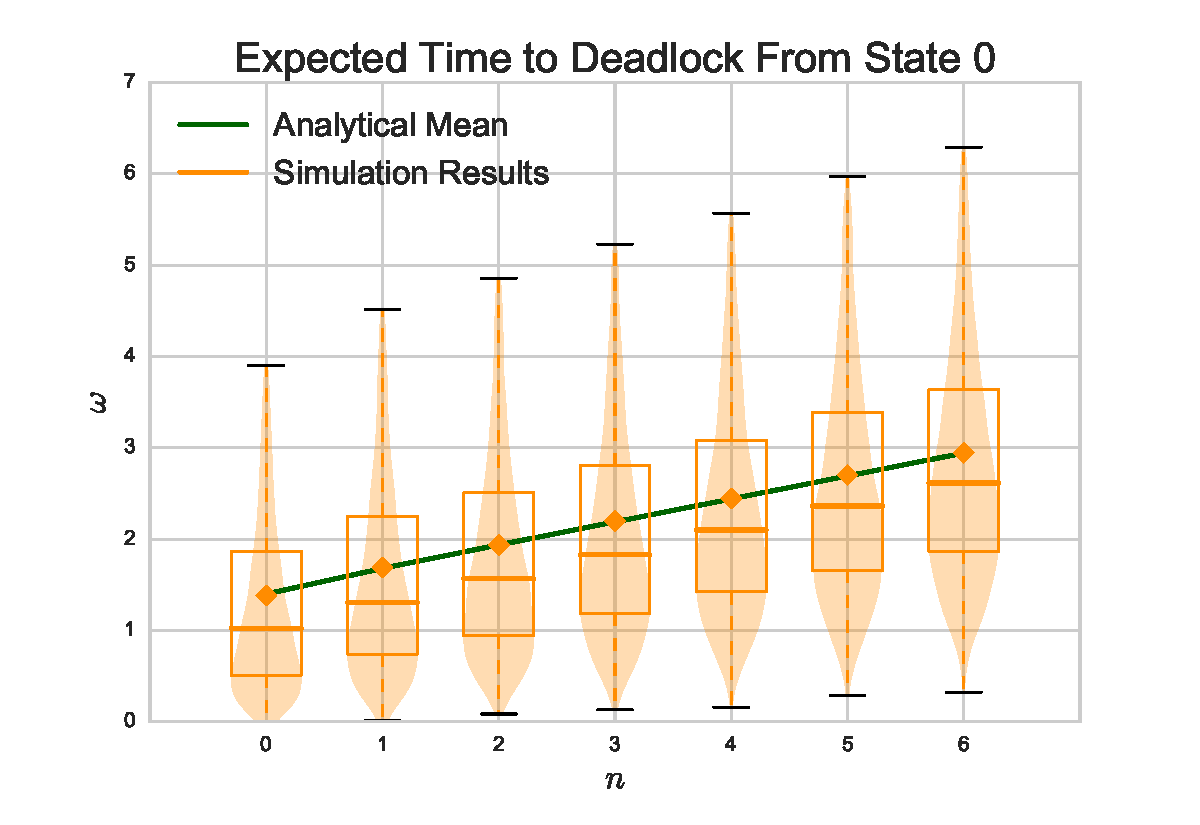
\includegraphics[width=0.7\textwidth]{img/mc_sim_vary_n_scheduled_vacations.pdf}
    \caption{Plot showing the time to deadlock of a system with scheduled vacations, comparing simulation and analytical results.}
    \label{fig:scheduled_vacations_MC_simulation}
\end{center}
\end{figure}


\subsection{Effect of Parameters of The Time to Deadlock with Vacations}

In order to enable further discussion of the CDF of the time to deadlock, let's define three periods during the schedule cycle of length $s + s_v$:

\begin{itemize}
    \item `Steady Period': during this period arrivals and services occur as usual, and the CDF increases steadily. Note that this does not imply a steady state.
    \item `Vacation Period': this is the period, lasting $s_v$ time units, where the server is on vacation. During these periods, the CDF remains constant.
    \item `Catch-up Period': this period occurs immediately after the server returns from vacation, after the system has had a chance to accept arrivals over the Vacation period, but not serve them. During this time the CDF shoots up, and then tails off into the Steady Period. The Steady period and the Catch-up Period lasts $s$ time units.
\end{itemize}

The height difference of the CDF during the Catch-up Period is effected by the amount the system fills up during the Vacation period. The length of the Catch-up Period is effected by how well the server can deal with the build up of customers caused by the vacation. If the server can deal with them well (for example because there is a high service rate) then the Catch-up Period will be short and will swiftly progress to a Steady Period, however if the server fails to cope, then the Catch-up Period will be long.

Figures~\ref{fig:cdf_varys} and \ref{fig:ttd_varys} show the effect of the time on duty, $s$ on the cdf of reaching deadlock and the expected time to deadlock. Figures~\ref{fig:cdf_varysv} and \ref{fig:ttd_varysv} show the effect of the vacation time, $s_v$ on the cdf of reaching deadlock and the expected time to deadlock. Increasing both $s$ and $s_v$ result in a fairly linear increase in the time to deadlock, however the behaviour of the system differs. Increasing $s$ allows a longer Steady Period in which the CDF increases slowly. Therefore at low values of $s$ the entire time the server is on duty is a Catch-up Period, however at high values of $s$ each period where the server is on duty is made up from a Catch-up Period and a Steady Period that increases as $s$ increases. As the CDF increases faster during the Catch-up Period, and at lower values of $s$ the system has a greater frequency of Catch-up Periods, then the CDF will increase more quickly for lower values of $s$, and so the expected time to deadlock is lower for lower values of $s$. On the other hand, increasing $s_v$ does not seem to have an effect on the height difference of the CDF during the Catch-up Period, and so increasing $s_v$ simply deplays the CDF from increasing. Therefore higher values of $s_v$ simply delay the effects of the system reaching deadlock, and so result in a longer time to deadlock.


\begin{figure}
\begin{center}
\begin{subfigure}[b]{0.45\textwidth}
    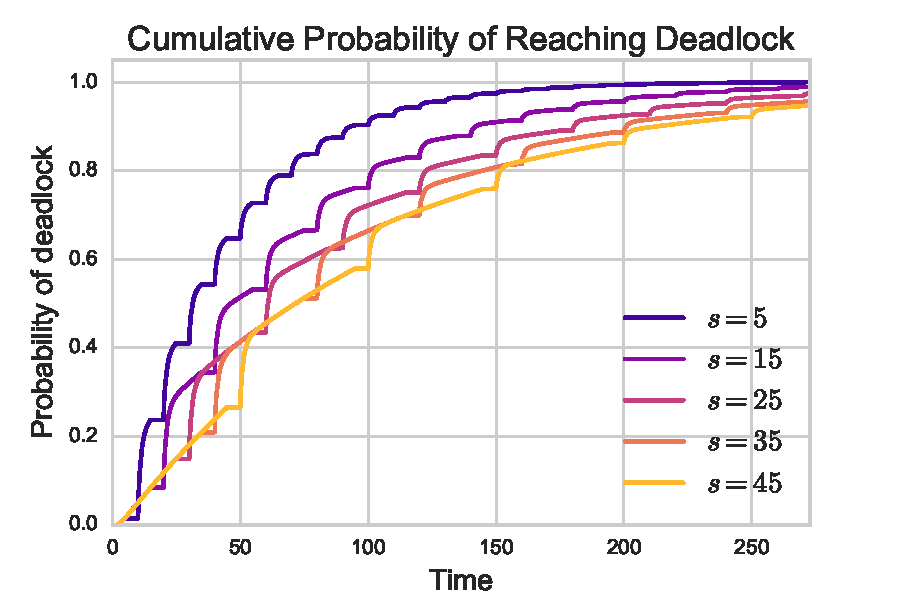
\includegraphics[width=\textwidth]{img/cdf_vary_s.pdf}
    \caption{Cumulative density function of reaching deadlock with vacations, varying $s$.}
    \label{fig:cdf_varys}
\end{subfigure}
\begin{subfigure}[b]{0.45\textwidth}
    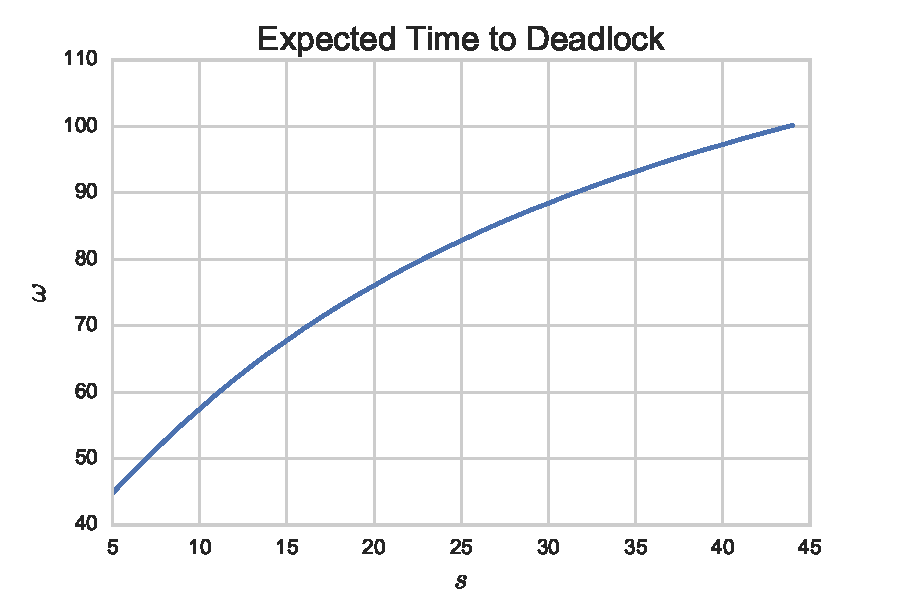
\includegraphics[width=\textwidth]{img/ttd_vary_s.pdf}
    \caption{Effect of varying $s$ on the time to deadlock.}
    \label{fig:ttd_varys}
\end{subfigure}
\end{center}
\caption{The effect of varying the time on duty, $s$, on the CDF and time to deadlock.}
\label{fig:ttdcdf_varys}
\end{figure}

\begin{figure}
\begin{center}
\begin{subfigure}[b]{0.45\textwidth}
    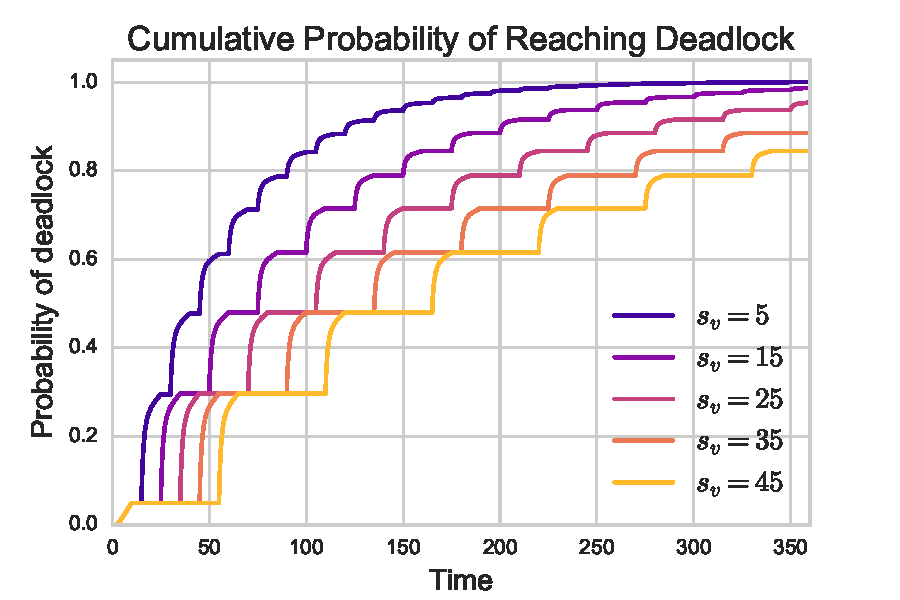
\includegraphics[width=\textwidth]{img/cdf_vary_sv.pdf}
    \caption{Cumulative density function of reaching deadlock with vacations, varying $s_v$.}
    \label{fig:cdf_varysv}
\end{subfigure}
\begin{subfigure}[b]{0.45\textwidth}
    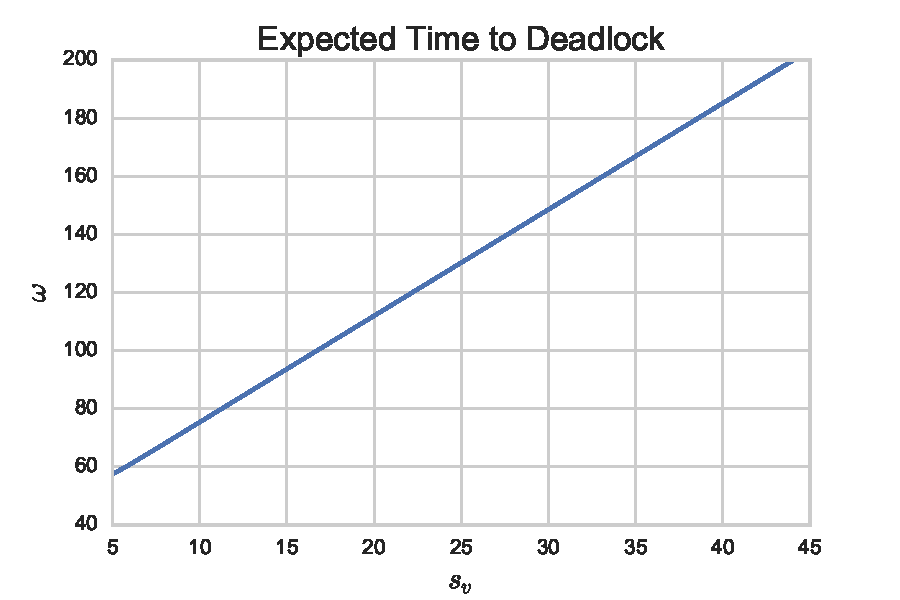
\includegraphics[width=\textwidth]{img/ttd_vary_sv.pdf}
    \caption{Effect of varying $s_v$ on the time to deadlock.}
    \label{fig:ttd_varysv}
\end{subfigure}
\end{center}
\caption{The effect of varying the vacation time, $s_v$, on the CDF and time to deadlock.}
\label{fig:ttdcdf_varysv}
\end{figure}

Figures~\ref{fig:cdf_varyn} and \ref{fig:ttd_varyn} show the effect of the queueing capacity, $n$ on the cdf of reaching deadlock and the expected time to deadlock. We see immediately that the height difference of the CDF during the Catch-up Period for smaller values of $n$ is much greater than for larger values. This is intuitive, as a queue with a smaller capacity will have greater chance of filling up during the Vacation Periods than a queue with lareger capacity. In addition the increase in CDF during the Steady Periods is steeper for smaller capacities, also intuitive as smaller capacities can fill up quicker than larger capacities, as mentioned in Chapter~\ref{chp:markovmodelsofdeadlock}.

\begin{figure}
\begin{center}
\begin{subfigure}[b]{0.45\textwidth}
    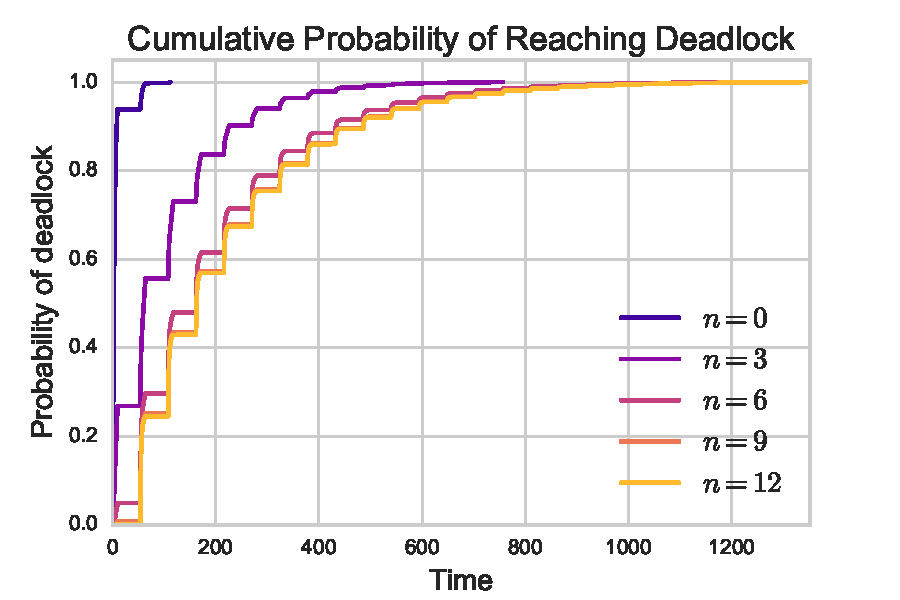
\includegraphics[width=\textwidth]{img/cdf_vary_n.pdf}
    \caption{Cumulative density function of reaching deadlock with vacations, varying $n$.}
    \label{fig:cdf_varyn}
\end{subfigure}
\begin{subfigure}[b]{0.45\textwidth}
    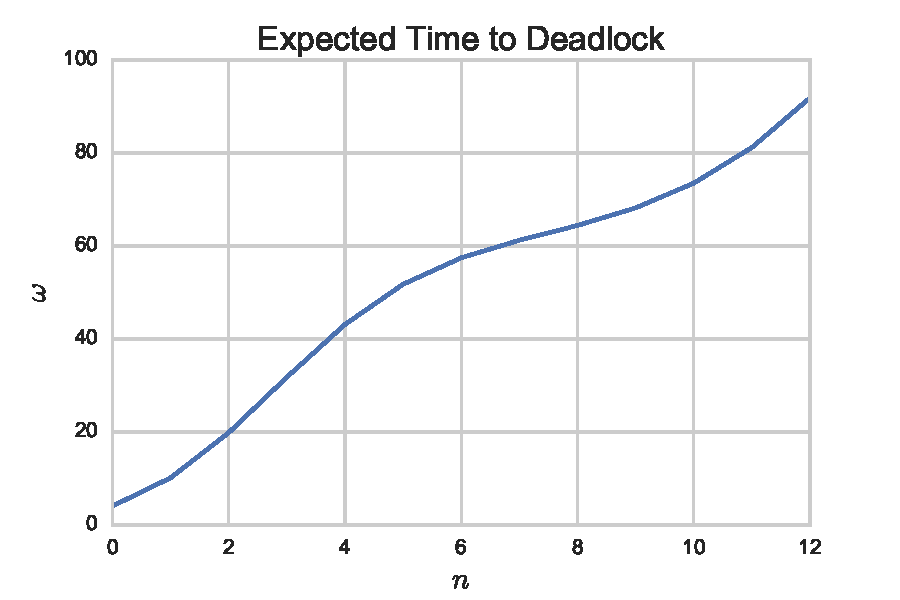
\includegraphics[width=\textwidth]{img/ttd_vary_n.pdf}
    \caption{Effect of varying $n$ on the time to deadlock.}
    \label{fig:ttd_varyn}
\end{subfigure}
\end{center}
\caption{The effect of varying the queueing capacity, $n$, on the CDF and time to deadlock.}
\label{fig:ttdcdf_varyn}
\end{figure}

Figures~\ref{fig:cdf_varymu} and \ref{fig:ttd_varymu} show the effect of the service rate, $\mu$ on the cdf of reaching deadlock and the expected time to deadlock. As with the case without scheduled vacations, as $\lim_{\mu \to 0} \omega = \infty$, and $\lim_{\mu \to \infty} \omega = \infty$, with a service time threshold in between where the time to deadlock is minimised. What is interesting is the difference in behaviour of the CDF of a system the $\mu_-$ and $\mu_+$, service rates either side of the threshold that yield similar expected times to deadlock. At $\mu_-$, the service rate to the left of the threshold, the service time is very long. Therefore it takes a long time for the first customer to finish service after the Vacation Period, and so the Catch-up Period takes a long time and increases slowly. At $\mu_+$ however, the service rate to the right of the threshold, the service rate is short, customers can leave the system quicker, and so the Catch-up Period is shorter and steeper, followed by a Steady Period in which the CDF does not increase much due to customers begin served so quickly.

\begin{figure}
\begin{center}
\begin{subfigure}[b]{0.45\textwidth}
    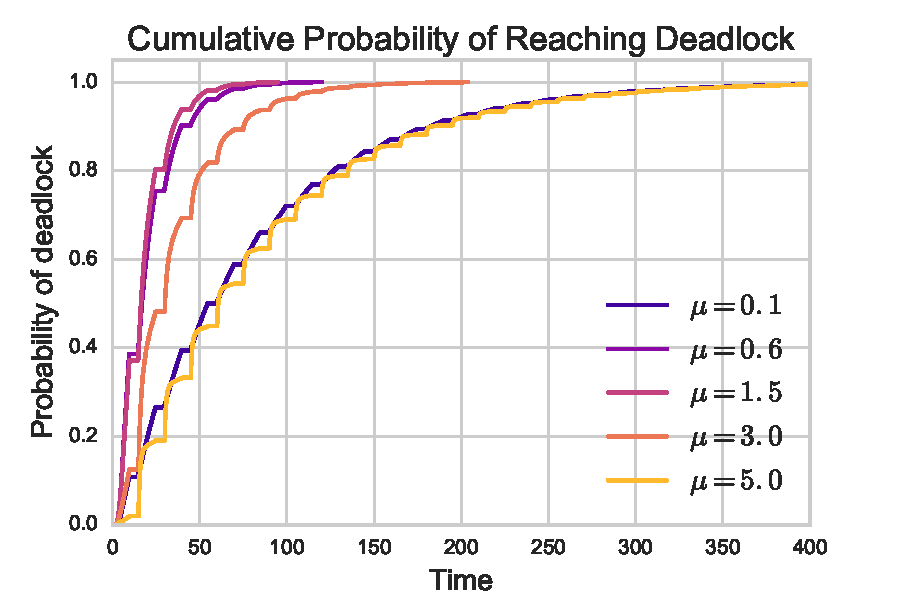
\includegraphics[width=\textwidth]{img/cdf_vary_mu.pdf}
    \caption{Cumulative density function of reaching deadlock with vacations, varying $\mu$.}
    \label{fig:cdf_varymu}
\end{subfigure}
\begin{subfigure}[b]{0.45\textwidth}
    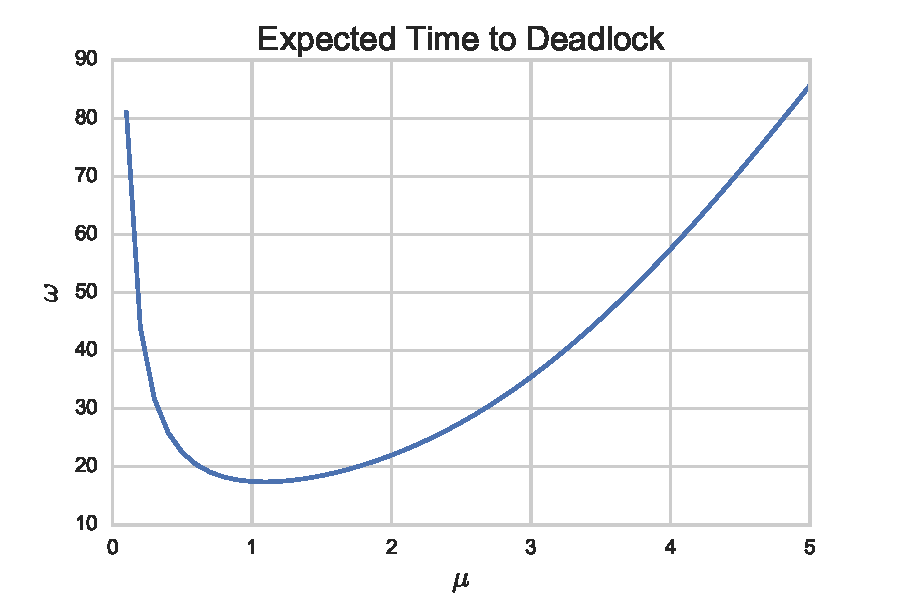
\includegraphics[width=\textwidth]{img/ttd_vary_mu.pdf}
    \caption{Effect of varying $\mu$ on the time to deadlock.}
    \label{fig:ttd_varymu}
\end{subfigure}
\end{center}
\caption{The effect of varying the service rate, $\mu$, on the CDF and time to deadlock.}
\label{fig:ttdcdf_varymu}
\end{figure}

Figures~\ref{fig:cdf_varyL} and \ref{fig:ttd_varyL} show the effect of the arrival rate, $\Lambda$ on the cdf of reaching deadlock and the expected time to deadlock, while Figures~\ref{fig:cdf_varyr11} and \ref{fig:ttd_varyr11} show the effect of the transition probability, $r_{11}$ on the cdf and time to deadlock. As discussed previously, increasing the arrival rate $\Lambda$ and the transition probability $r_{11}$ decreases the time to deadlock. Looking at the CDF, higher arrival rates and transition probabilities lead to a greater jump in the CFD during the Catch-up Periods. For increasing the arrival rate, this is due to the queue filling up it's capacity quicker during the Vacation Period, and there is a higher probability of a fuller queue at the end of the server's vacation. For increasing transition probability however, the arrivals during the Vacation Period stay constant (as there are no services to cause rejoins during this time); the increase in CDF during the Catch-up Period is due to the probability of a rejoin, and hence a blockage and then deadlock, immediately after the Vacation Period once the queue has had chance to fill is increases as the transition probability increases.

\begin{figure}
\begin{center}
\begin{subfigure}[b]{0.45\textwidth}
    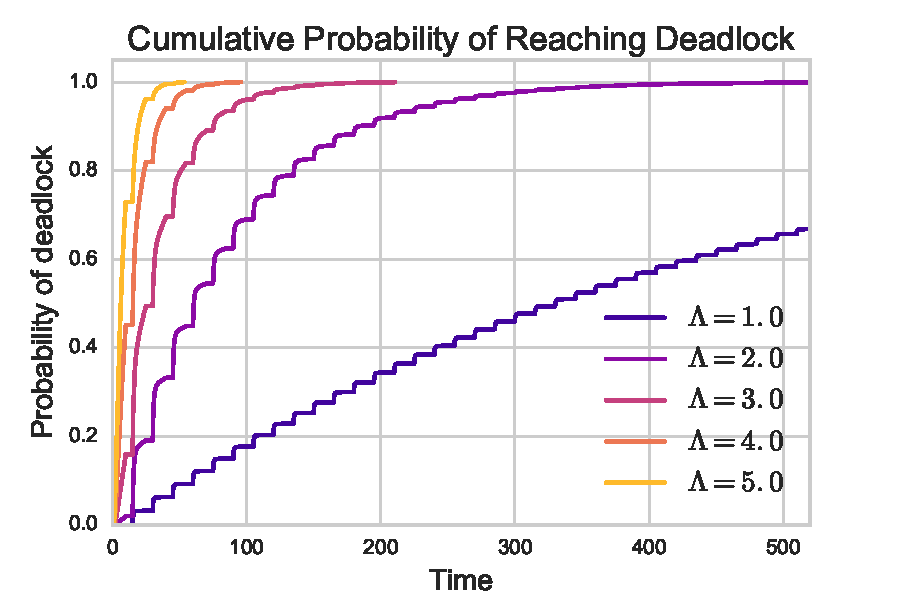
\includegraphics[width=\textwidth]{img/cdf_vary_L.pdf}
    \caption{Cumulative density function of reaching deadlock with vacations, varying $\Lambda$.}
    \label{fig:cdf_varyL}
\end{subfigure}
\begin{subfigure}[b]{0.45\textwidth}
    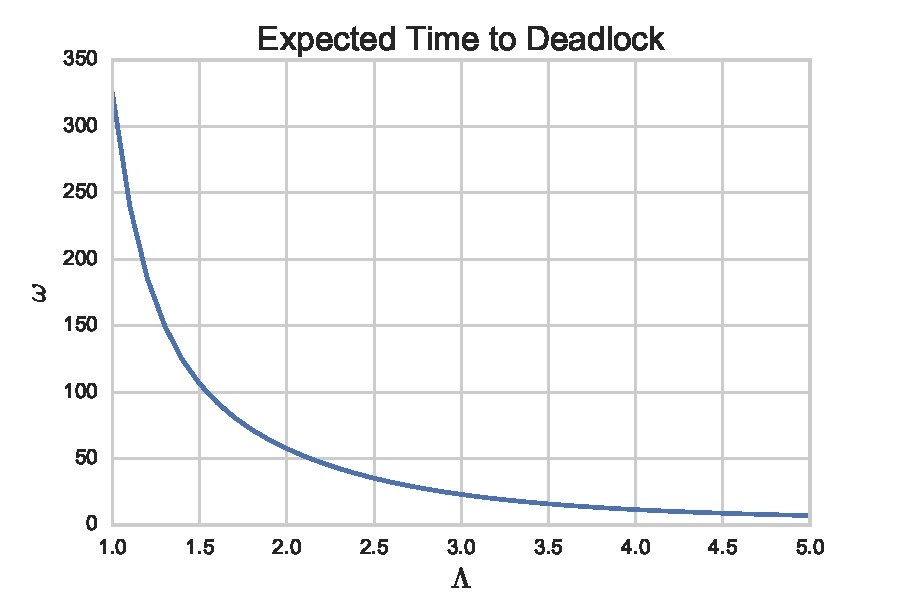
\includegraphics[width=\textwidth]{img/ttd_vary_L.pdf}
    \caption{Effect of varying $\Lambda$ on the time to deadlock.}
    \label{fig:ttd_varyL}
\end{subfigure}
\end{center}
\caption{The effect of varying the arrival rate, $\Lambda$, on the CDF and time to deadlock.}
\label{fig:ttdcdf_varyL}
\end{figure}


\begin{figure}
\begin{center}
\begin{subfigure}[b]{0.45\textwidth}
    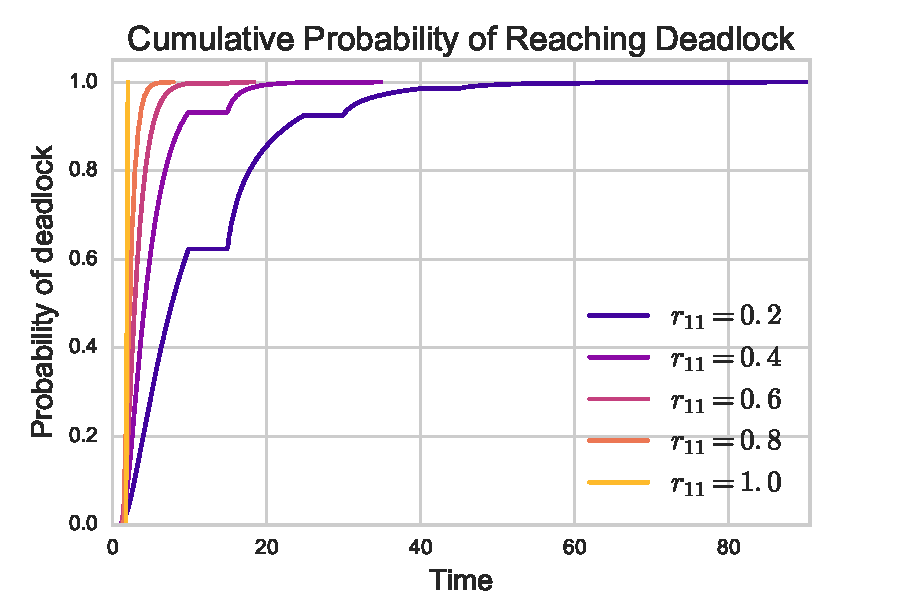
\includegraphics[width=\textwidth]{img/cdf_vary_r11.pdf}
    \caption{Cumulative density function of reaching deadlock with vacations, varying $r_{11}$.}
    \label{fig:cdf_varyr11}
\end{subfigure}
\begin{subfigure}[b]{0.45\textwidth}
    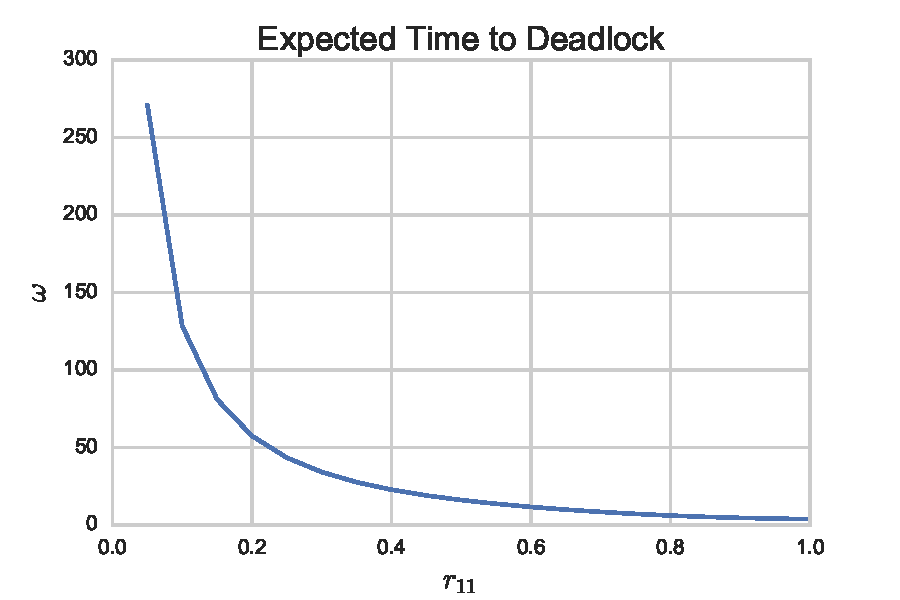
\includegraphics[width=\textwidth]{img/ttd_vary_r11.pdf}
    \caption{Effect of varying $r_{11}$ on the time to deadlock.}
    \label{fig:ttd_varyr11}
\end{subfigure}
\end{center}
\caption{The effect of varying the transition probability, $r_{11}$, on the CDF and time to deadlock.}
\label{fig:ttdcdf_varyr11}
\end{figure}

\bibliographystyle{plain}
\bibliography{refs}

\end{document}
